% Бүлэг 1

\chapter{Бизнес эрхлэгчдийн сурталчилгааны нэгдсэн вебийн судалгаа} % Бүлгийн нэр
\label{Chapter1} % Энэ бүлэг рүү ишлэл хийх бол \ref{Chapter1} командыг ашигла 

%-------------------------------------------------------------------------------

% Агуулгад ашигласан хэвшүүлэлтийн зарим командын тодорхойлолт
\newcommand{\keyword}[1]{\textbf{#1}}
\newcommand{\tabhead}[1]{\textbf{#1}}
\newcommand{\code}[1]{\texttt{#1}}
\newcommand{\file}[1]{\texttt{\bfseries#1}}
\newcommand{\option}[1]{\texttt{\itshape#1}}

%-------------------------------------------------------------------------------

\LaTeX{} ашиглаж тезис бичих энэхүү гоёмсог, ашиглахад хялбарт загварт тавтай морилно уу. 

Хэрэв таны бичиж байгаа (бичихээр төлөвлөсөн) тезис техникийн эсвэл математикийн чиглэлээр бол \LaTeX{} ашиглахыг зөвлөж байна. Учир нь текст процессор дээр загвараа гаргах гэж цаг алдалгүй зөвхөн бичих зүйлдээ анхаарахад л болно.

\LaTeX{} бол хэдэн зуу, мянган хуудастай баримт бичгийг мэргэжлийн түвшинд хялбархан гаргаж чаддаг. Энгийн командын тусламжтай гарчиг, хуудасны зах, толгой болон хөлийг автоматаар үүсгэж форматын нэгдмэл байдал, үзэмжийг хангадаг. Түүний нэг гол хүч чадал нь \emph{хүнд} математикийг ч амархан бичиж чадна.

%-------------------------------------------------------------------------------
\section{Хэрэглэгчийн судалгаа}
Бизнес эрхлэгчдийн сурталчилгааны нэгдсэн вебийн хэрэглэгчдийн судалгааг 2016-оны 9-сарын 25-с 2016-оны 10-сарын 02-ны өдөр хүртэл 45 хүнээс авсан судалгаа.
%-------------------------------------------------------------------------------
\begin{figure}[htbp]
	\centering
	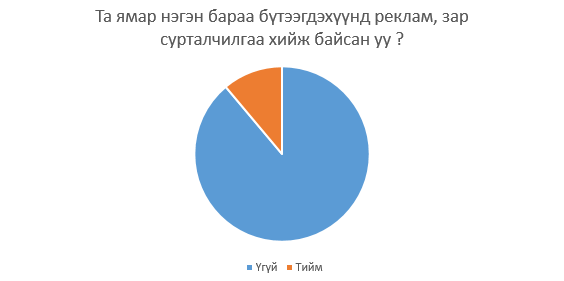
\includegraphics[scale=0.7]{Chart/Chart1}
	\caption[Хэрэглэгчийн судалгаа]{Реклам сурталчилгаа хийж байсан бэ?(Асуулга.)}
	\label{fig:Chart1}
\end{figure}

\begin{figure}[htbp]
	\centering
	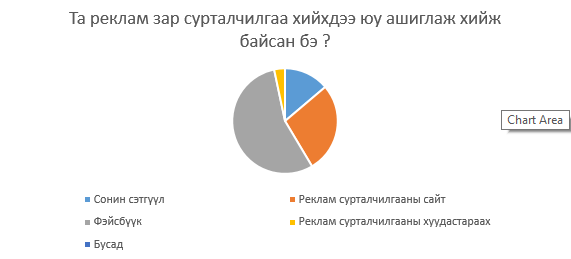
\includegraphics[scale=0.7]{Chart/Chart2}
	\caption[Хэрэглэгчийн судалгаа]{Реклам сурталчилгаа хийхдээ юу ашиглаж байсан бэ?(Асуулга.)}
	\label{fig:Chart2}
\end{figure}

\begin{figure}[htbp]
	\centering
	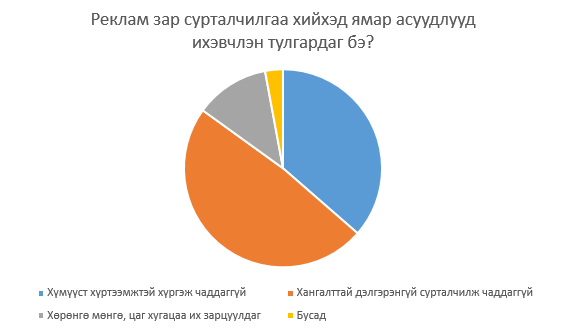
\includegraphics[scale=0.7]{Chart/Chart3}
	\caption[Хэрэглэгчийн судалгаа]{Тулгардаг асуудлууд(Асуулга.)}
	\label{fig:Chart3}
\end{figure}

\begin{figure}[htbp]
	\centering
	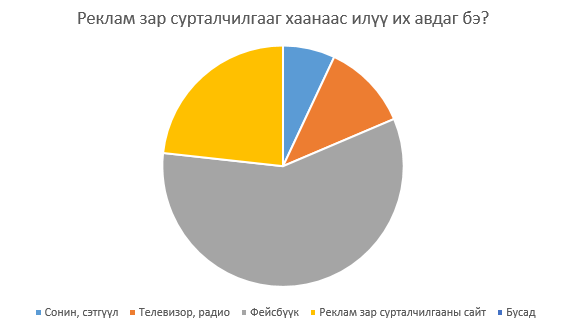
\includegraphics[scale=0.7]{Chart/Chart4}
	\caption[Хэрэглэгчийн судалгаа]{Реклам сурталчилгааг хаанаас авдаг бэ?(Асуулга.)}
	\label{fig:Chart4}
\end{figure}
\begin{figure}[htbp]
	\centering
	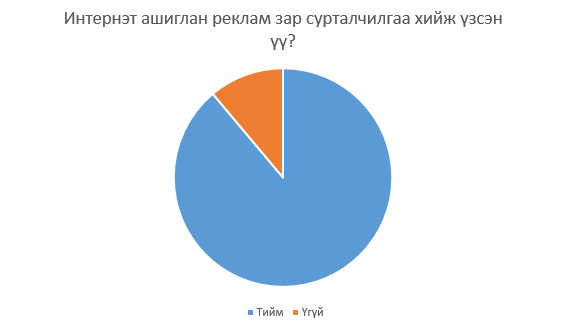
\includegraphics[scale=0.7]{Chart/Chart5}
	\caption[Хэрэглэгчийн судалгаа]{Интернэт ашиглан реклам хийж байсан уу?(Асуулга.)}
	\label{fig:Chart5}
\end{figure}

\begin{figure}[htbp]
	\centering
	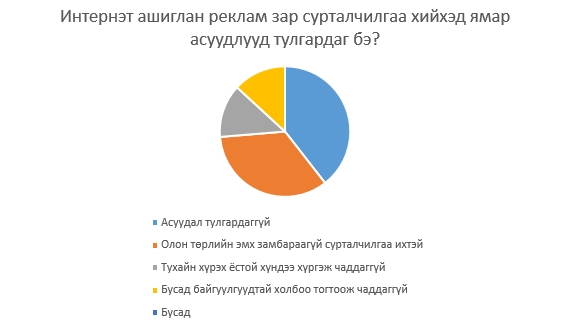
\includegraphics[scale=0.7]{Chart/Chart6}
	\caption[Интернэт ашиглан сурталчилгаа хийхэд тулгардаг асуудлууд]{Интернэт ашиглан сурталчилгаа хийхэд тулгардаг асуудлууд(Асуулга.)}
	\label{fig:Chart6}
\end{figure}

\begin{figure}[htbp]
	\centering
	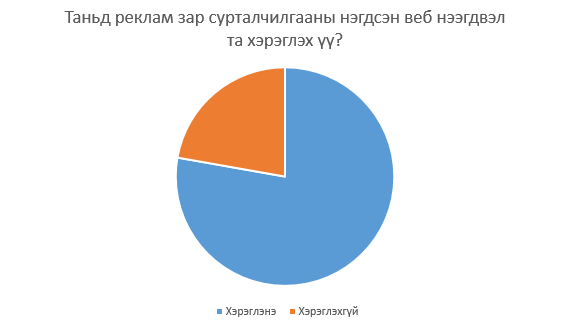
\includegraphics[scale=0.7]{Chart/Chart7}
	\caption[Хэрэглэгчийн судалгаа]{Сурталчилгааны веб нээгдвэл ашиглах эсэх(Асуулга.)}
	\label{fig:Chart7}
\end{figure}

%-------------------------------------------------------------------------------
\section{Хөгжүүлэлтэд ашиглах алгоритм}

\LaTeX{} бол Microsoft Word, Adobe Pages шиг \textsc{WYSIWYG} (Таны Харж байгаа Зүйл бол Таны Оруулсан Зүйл) төрлийн текст боловсруулах програм биш. \LaTeX{} --д зориулсан баримт нь үнэндээ \emph{хэвшүүлээгүй} задгай текст бүхий файл юм. Өөрийн тексттэй хамт түүнийг хэрхэн хэвшүүлэхийг тухай энгийн командыг бичиж, энэ файлаар \LaTeX{} --т хэлж өгдөг. Жишээ нь \emph{текстийг налуу болгож тодотгохдоо} \verb|\emph{text}| командыг ашиглах ба налуу болгох текстээ их хаалтанд бичнэ. Өөрөөр хэлбэл \LaTeX{} нь HTML -тэй маш төстэй ''{mark-up}'' хэл юм.

%-------------------------------------------------------------------------------

\section{Технологийн судалгаа}

\section{Laravel фреймворк}
Ларавел фреймворк нь  MVC вэб програмуудын хөгужилд зориулагдсан үнэгүй, нээлттэй эхтэй PHP вэб фреймворк юм. Ларавел нь MIT тусгай зөвшөөрөлтэй бөгөөд GitHub дээр байршдаг. PHP орчинд алдартай 2013 оны 12 сарын судалгаагаар Laravel  2014 оны хувьд хамгийн ирээдүйтэй PHP вэб фреймворк гэж судлагдсан байдаг.
PHP фреймворкүүдийг 2015 оны эцсийн байдлаар харьцуулж үзэхэд  хамгийн их хэрэглэгддэг фреймворк гэдэг нь судалгаагаар тогтоогдсон.

\section{MySQL}
MySQL нь холбоост өгөгдлийн санг удирдах систем юм. MySQL хэмээх нэрний хувьд уг системийг санаачлан хөгжүүлэгч Micheal Widenius-ын охины нэр My + SQL(Structed Query Language) гэсэн утгатай ажээ.
Энэ систем нь GNU (General Public License) буюу нээлтэй эхийн систем учир хүссэн хэн бүхэн хөгжүүлэлтэнд оролцож, үнэгүй хэрэглэж болох юм. Эзэмшигч нь алдарт Java-г хөгжүүлсэн Sun MicroSystems компани байсан ба, одоогоор Sun-г Oracle корпораци эзэмших болсон билээ.
Үнэгүй програм хангамжийн өгөгдлийн санг удирдах системд ихэвчлэн MySQL-ийг хэрэглэдэг бөгөөд тэдгээрийн сонгодог жишээ гэвэл Joomla, Drupal, Wordpress, phpBB гэх мэт агуулга удирдах системүүд (CMS-Content Management System), Wikipedia, Facebook, Google гэх мэт томоохон компаниуд хэрэглэдэг юм.
Хөгжүүлэлт нь C/C++ хэл дээр хийгдсэн ба AIX, BSDi, FreeBSD, HP-UX, i5/OS, Linux, Mac OS X, NetBSD, Novell NetWare, OpenBSD, OpenSolaris, eComStation, OS/2 Warp, QNX, IRIX, Solaris, Symbian, SunOS, SCO OpenServer, SCO UnixWare, Sanos, Tru64, Microsoft Windows гэсэн олон үйлдлийн системүүд дээр ажилладаг.
MySQL бол хамгийн өргөн хэрэглээтэй нээлттэй эхийн (Open Source) өгөгдлийн сан удирдах програм юм. Анх 1995 онд зах зээлд гарсан ба с/с++ хэл дээр бичигдсэн. Одоогийн байдлаар 5.7 нь хамгийн сүүлийн хувилбар болон гараад байна. Энэ сүүлийн хувилбар дээр нэмэгдсэн давуу талууд гэвэл 3 дахин хурдан үйл ажиллагаатай болсон мөн натив JSON дэмжигчтэй болсон гэх мэт шинэлэг үйлдлүүд нэмэгдсэн байна.

\section{Php}
  Rasmus Lerdorf WWW-д вэб хуудас үүсгэх үедээ өгөгдөл боловсруулах хялбархан арга хайж байгаад 1995 онд PHP хэлийг скрипт хэл байдлаар зохиосон.
PHP нь сервер талын скрипт хэл ба динамик вэб хуудас хийхэд илүү тохиромжтой. Энэ скрипт хэл нь энгийн хэрэглээний вэб сайтаас эхлээд байгууллагын иж бүрэн вэб программ хийж болохоор MySQL мэтийн өгөгдлийн сантай харилцан ажиллах боломжтой.
Хуудас ачаалах үед броузерээр нэг бүрчлэн уншдаг HTML-тэй адилгүй, PHP баримтыг бэлтгэхдээ серверээр урьдчилан боловсруулдаг. PHP код агуулсан хуудас нь хэрэглэгчийн броузерт илгээгдхээс өмнө серверээр боловсруулагдсан байдаг.
PHP хэлний өөр нэг давуу тал бол скриптэн хэл юм. Ихэнх програмчлалын хэлнүүдэд ажиллахын өмнө машины хэл рүү хөрвүүлэх тусгай файлууд /compile/ шаардлагатай байдаг бол PHP хэлний хувьд хөрвүүлэлт хийх шаардлагагүй байдаг тул код засварлах болон шалгахад илүү хурдан байдаг

\section{JQuery}
2006 оны эхээр АНУ-ын Нью-Иорк хотын BarCamp-д John Resig хэмээх вэб хөгжүүлэгч залуу jQuery сангийн тухай анх мэдэгджээ. Resig өөрийн вэб сайтдаа: Тухайн үед байгаа сангуудад сэтгэл дундуур байгаагаа, мөн түүнчлэн JavaScript – ий тухай бичилтийг нь багасгаснаар маш их ажил хөнгөвчлөх боломжтой, энгийн үйлдлүүдэд зориулан тусгай хэрэгслүүд нэмэх хэрэгтэй гэж дурдсан байдаг.
Хөгжүүлэх нийгэмлэгт jQuery нь томоохон амжилт авчирсан төдийгүй улмаар маш хурдтай хөгжсөн. Бусад хөгжүүлэгчид сан боловсронгуй болгоход тусалж эхэлснээр jQuery – гийн анхны хувилбар 1.0 нь 2006 оны 8-р сарын 26- нд гарсан.
Түүнээс хойш jQuery 3.1.1 хувилбар гарсан ба хөгжүүлэлтийн нийгэмлэгээс plug-in –ийг маш ихээр оруулсан. Plug-in нь jQuery – ийн сангийн цөм хэсэг биш харин нэмэлт хэрэгсэл юм. 
jQuery – гийн давуу талууд нь:
\begin{itemize}
\item Файлын хэмжээ бага
\item Маш энгийн бичилттэй
\item Холбоо бүхий method – уудтай
\item Санг өргөтгөх plug-in нь энгийн бүтэцтэй
\item Асар том онлайн нийгэмлэгтэй
\item JQueryUI мэтийн jQuery – гийн нэмэлт сонголтуудтай
\end{itemize}
\section{Service}
2006 оны эхээр АНУ-ын Нью-Иорк хотын BarCamp-д John Resig хэмээх вэб хөгжүүлэгч залуу jQuery сангийн тухай анх мэдэгджээ. Resig өөрийн вэб сайтдаа: Тухайн үед байгаа сангуудад сэтгэл дундуур байгаагаа, мөн түүнчлэн JavaScript – ий тухай бичилтийг нь багасгаснаар маш их ажил хөнгөвчлөх боломжтой, энгийн үйлдлүүдэд зориулан тусгай хэрэгслүүд нэмэх хэрэгтэй гэж дурдсан байдаг.
Хөгжүүлэх нийгэмлэгт jQuery нь томоохон амжилт авчирсан төдийгүй улмаар маш хурдтай хөгжсөн. Бусад хөгжүүлэгчид сан боловсронгуй болгоход тусалж эхэлснээр jQuery – гийн анхны хувилбар 1.0 нь 2006 оны 8-р сарын 26- нд гарсан.
Түүнээс хойш jQuery 3.1.1 хувилбар гарсан ба хөгжүүлэлтийн нийгэмлэгээс plug-in –ийг маш ихээр оруулсан. Plug-in нь jQuery – ийн сангийн цөм хэсэг биш харин нэмэлт хэрэгсэл юм. 
jQuery – гийн давуу талууд нь:
\begin{itemize}
\item Файлын хэмжээ бага
\item Маш энгийн бичилттэй
\item Холбоо бүхий method – уудтай
\item Санг өргөтгөх plug-in нь энгийн бүтэцтэй
\item Асар том онлайн нийгэмлэгтэй
\item JQueryUI мэтийн jQuery – гийн нэмэлт сонголтуудтай
\end{itemize}
\section{Бүлгийн дүгнэлт}
%-------------------------------------------------------------------------------